% answers.tex —— 1977 年·江苏南京市初试卷 · 参考答案与详细解析片段
% 由 tools/generate_projects.py 依来源总账自 1977/1977_数学真题_江苏南京市初试_试题.md + 1977/1977_数学真题_江苏南京市初试_解析正文.md + 1977/1977_数学真题_江苏南京市初试_答案要点.md 生成，勿手改（改源 MD 后重跑）


\begin{gktip}
固定源为两页纯题面扫描（原书页码 230 起），未附解答。下文各题由编者独立推导。原卷大题号「一、……十、」已转写为阿拉伯数字；题一、二、四的小题「1．2．…」与题十的「①②③」统一为「（N）」，未增删题干。
\end{gktip}

\begin{answer}
\gksolhead{1}{}

\textbf{题目}：

写出下列各题的正确结果：

（1） $\sqrt{\left(\sqrt{2}-\sqrt{3}\right)^{2}}$；

（2） $0.2^{7}\times5^{7}$；

（3） $\log_{3}27^{-1}$；

（4） $\operatorname{tg}10^{\circ}\operatorname{tg}20^{\circ}\operatorname{tg}70^{\circ}\operatorname{tg}80^{\circ}$。

\Needspace{4\baselineskip}
\textbf{解析}

\gksubpart{（1）}

\Needspace{5\baselineskip}
因 $\sqrt{2}<\sqrt{3}$，$\sqrt{2}-\sqrt{3}<0$，故

\nopagebreak[4]
\[
\sqrt{\left(\sqrt{2}-\sqrt{3}\right)^{2}}
=\left|\sqrt{2}-\sqrt{3}\right|
=\sqrt{3}-\sqrt{2}.
\]

\gksubpart{（2）}

\nopagebreak[4]
\[
0.2^{7}\times5^{7}=(0.2\times5)^{7}=1^{7}=1.
\]

\gksubpart{（3）}

\nopagebreak[4]
\[
\log_{3}27^{-1}=\log_{3}3^{-3}=-3.
\]

\gksubpart{（4）}

\Needspace{5\baselineskip}
$\operatorname{tg}70^{\circ}=\cot20^{\circ}$，$\operatorname{tg}80^{\circ}=\cot10^{\circ}$，故

\nopagebreak[4]
\[
\operatorname{tg}10^{\circ}\operatorname{tg}20^{\circ}\operatorname{tg}70^{\circ}\operatorname{tg}80^{\circ}
=(\operatorname{tg}10^{\circ}\cot10^{\circ})(\operatorname{tg}20^{\circ}\cot20^{\circ})=1.
\]

\gkanswer{答案（1）：$\sqrt{3}-\sqrt{2}$。}

\gkanswer{答案（2）：$1$。}

\gkanswer{答案（3）：$-3$。}

\gkanswer{答案（4）：$1$。}

\end{answer}
\begin{answer}
\gksolhead{2}{}

\textbf{题目}：

用“$<$”或“$>$”符号把下列各组的值连结起来：

（1） $\log_{2}\dfrac{3.14}{\pi}$ 与 $0$；

（2） $\cos40^{\circ}$ 与 $\sin40^{\circ}$；

（3） $\left(\dfrac{2}{5}\right)^{-\frac{2}{3}}$ 与 $\left(\dfrac{2}{5}\right)^{-\frac{1}{2}}$；

（4） $0.\dot{3}$ 与 $\dfrac{3}{10}$。

\Needspace{4\baselineskip}
\textbf{解析}

\gksubpart{（1）}

\Needspace{5\baselineskip}
$\pi>3.14$，故 $0<\dfrac{3.14}{\pi}<1$，从而

\nopagebreak[4]
\[
\log_{2}\dfrac{3.14}{\pi}<\log_{2}1=0.
\]

\gksubpart{（2）}

\Needspace{5\baselineskip}
$\sin40^{\circ}=\cos50^{\circ}$，而 $[0^{\circ},90^{\circ}]$ 上余弦单调递减且 $40^{\circ}<50^{\circ}$，故 $\cos40^{\circ}>\cos50^{\circ}$，即

\nopagebreak[4]
\[
\cos40^{\circ}>\sin40^{\circ}.
\]

\gksubpart{（3）}

\Needspace{5\baselineskip}
底数 $\dfrac{2}{5}\in(0,1)$，指数函数单调递减；又 $-\dfrac{2}{3}<-\dfrac{1}{2}$，故

\nopagebreak[4]
\[
\left(\dfrac{2}{5}\right)^{-\frac{2}{3}}>\left(\dfrac{2}{5}\right)^{-\frac{1}{2}}.
\]

\gksubpart{（4）}

\Needspace{5\baselineskip}
$0.\dot{3}=0.333\cdots=\dfrac{1}{3}>\dfrac{3}{10}$，故

\nopagebreak[4]
\[
0.\dot{3}>\dfrac{3}{10}.
\]

\gkanswer{答案（1）：$\log_{2}\dfrac{3.14}{\pi}<0$。}

\gkanswer{答案（2）：$\cos40^{\circ}>\sin40^{\circ}$。}

\gkanswer{答案（3）：$\left(\dfrac{2}{5}\right)^{-\frac{2}{3}}>\left(\dfrac{2}{5}\right)^{-\frac{1}{2}}$。}

\gkanswer{答案（4）：$0.\dot{3}>\dfrac{3}{10}$。}

\end{answer}
\begin{answer}
\gksolhead{3}{}

\textbf{题目}：

求 $\sin165^{\circ}$ 与 $\cos255^{\circ}$ 的值。

\Needspace{4\baselineskip}
\textbf{解析}

\nopagebreak[4]
\[
\sin165^{\circ}=\sin(180^{\circ}-15^{\circ})=\sin15^{\circ}
=\sin(45^{\circ}-30^{\circ})
=\dfrac{\sqrt{6}-\sqrt{2}}{4}.
\]

\nopagebreak[4]
\[
\cos255^{\circ}=\cos(180^{\circ}+75^{\circ})=-\cos75^{\circ}
=-\sin15^{\circ}
=-\dfrac{\sqrt{6}-\sqrt{2}}{4}.
\]

\gkanswer{答案：$\sin165^{\circ}=\dfrac{\sqrt{6}-\sqrt{2}}{4}$，$\cos255^{\circ}=-\dfrac{\sqrt{6}-\sqrt{2}}{4}$。}

\end{answer}
\begin{answer}
\gksolhead{4}{}

\textbf{题目}：

求极限值：

\Needspace{5\baselineskip}
（1） 

\nopagebreak[4]
\[
\lim_{x\to2}\frac{2x^{2}-3x-2}{x-2}\text{\text{；}}
\]

\Needspace{5\baselineskip}
（2） 

\nopagebreak[4]
\[
\lim_{x\to\infty}\frac{3x^{2}-4x+5}{2x^{2}+x-1}\text{。}
\]

\Needspace{4\baselineskip}
\textbf{解析}

\gksubpart{（1）}

\Needspace{5\baselineskip}
分子因式分解 $2x^{2}-3x-2=(2x+1)(x-2)$，$x\to2$ 时 $x-2\ne0$，约去后

\nopagebreak[4]
\[
\lim_{x\to2}\frac{2x^{2}-3x-2}{x-2}
=\lim_{x\to2}(2x+1)=5.
\]

\gksubpart{（2）}

\Needspace{5\baselineskip}
分子、分母同除以 $x^{2}$：

\nopagebreak[4]
\[
\lim_{x\to\infty}\frac{3x^{2}-4x+5}{2x^{2}+x-1}
=\lim_{x\to\infty}\frac{3-\dfrac{4}{x}+\dfrac{5}{x^{2}}}{2+\dfrac{1}{x}-\dfrac{1}{x^{2}}}
=\dfrac{3}{2}.
\]

\gkanswer{答案（1）：$5$。}

\gkanswer{答案（2）：$\dfrac{3}{2}$。}

\end{answer}
\begin{answer}
\gksolhead{5}{}

\textbf{题目}：

\Needspace{5\baselineskip}
解方程组

\nopagebreak[4]
\[
\begin{cases}
\dfrac{3x-5y}{2xy}=1\dfrac{1}{3}\\[8pt]
\dfrac{3}{x}+\dfrac{1}{y}=4
\end{cases}
\]

\Needspace{4\baselineskip}
\textbf{解析}

\Needspace{5\baselineskip}
由分母非零知 $x,y\ne0$。令 $u=\dfrac{1}{x}$，$v=\dfrac{1}{y}$，方程组化为

\nopagebreak[4]
\[
\begin{cases}
\dfrac{3}{2}v-\dfrac{5}{2}u=\dfrac{4}{3}\\[6pt]
3u+v=4
\end{cases}
\]

\Needspace{5\baselineskip}
由第二式 $v=4-3u$，代入第一式：

\nopagebreak[4]
\[
6-\frac{9}{2}u-\frac{5}{2}u=\frac{4}{3}
\quad\Longrightarrow\quad
6-7u=\frac{4}{3}
\quad\Longrightarrow\quad
u=\frac{2}{3}.
\]

\Needspace{5\baselineskip}
从而 $v=4-3\times\dfrac{2}{3}=2$，即

\nopagebreak[4]
\[
x=\frac{3}{2},\qquad y=\frac{1}{2}.
\]

验根：$\dfrac{3}{x}+\dfrac{1}{y}=2+2=4$；$\dfrac{3x-5y}{2xy}=\dfrac{2}{\dfrac{3}{2}}=\dfrac{4}{3}=1\dfrac{1}{3}$，均满足原方程组。

\gkanswer{答案：$x=\dfrac{3}{2}$，$y=\dfrac{1}{2}$。}

\end{answer}
\begin{answer}
\gksolhead{6}{}

\textbf{题目}：

在 $\odot O$ 中，直径 $AB$ 和弦 $AC$ 的夹角为 $15^{\circ}$，过 $C$ 点的切线和 $AB$ 的延长线相交于 $P$，已知 $OP=24\,\mathrm{cm}$，求 $\odot O$ 的半径。

\begin{gktip}
原源 PDF 第 2 页附有圆与切线的示意图；LaTeX 版按源图重绘。
\end{gktip}
\nopagebreak[4]
\begin{center}% 1977 年江苏南京市初试卷第六题：圆 O 中直径 AB 与弦 AC 的夹角 15°，过 C 的切线交 AB 延长线于 P，OP=24cm（按源卷第 2 页布局；r=2，OP=2/\cos30°≈2.309，P 在 B 右侧）
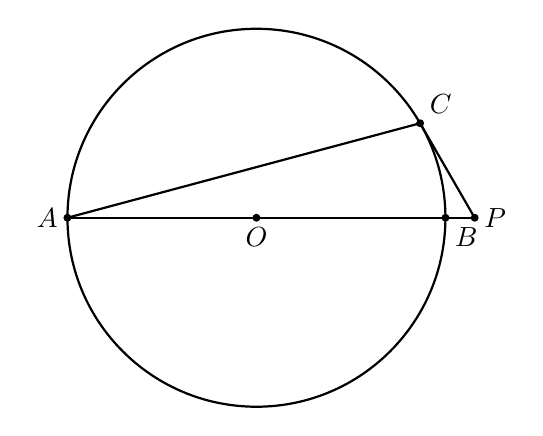
\begin{tikzpicture}[scale=1.2]
  \coordinate (O) at (0,0);
  \coordinate (A) at (-2,0);
  \coordinate (B) at (2,0);
  \coordinate (C) at (1.732,1);
  \coordinate (P) at (2.309,0);
  \draw[thick] (O) circle (2);
  \draw[thick] (A)--(P);
  \draw[thick] (A)--(C);
  \draw[thick] (C)--(P);
  \fill (O) circle (1.2pt) node[below] {$O$};
  \fill (A) circle (1.2pt) node[left] {$A$};
  \fill (B) circle (1.2pt) node[below right] {$B$};
  \fill (C) circle (1.2pt) node[above right] {$C$};
  \fill (P) circle (1.2pt) node[right] {$P$};
\end{tikzpicture}
\end{center}
\nopagebreak[4]
\Needspace{4\baselineskip}
\textbf{解析}

\Needspace{5\baselineskip}
连接 $OC$。因 $OA=OC$（同为半径），$\angle OAC=\angle OCA=15^{\circ}$，故

\nopagebreak[4]
\[
\angle AOC=180^{\circ}-2\times15^{\circ}=150^{\circ},
\qquad
\angle COP=180^{\circ}-150^{\circ}=30^{\circ}.
\]

\Needspace{5\baselineskip}
$CP$ 为过 $C$ 的切线，故 $OC\perp CP$，$\angle OCP=90^{\circ}$。在 $\mathrm{Rt}\triangle OCP$ 中，

\nopagebreak[4]
\[
\cos30^{\circ}=\frac{OC}{OP}=\frac{r}{24}
\quad\Longrightarrow\quad
r=24\cos30^{\circ}=12\sqrt{3}\ (\mathrm{cm}).
\]
\nopagebreak[4]
\begin{center}% 1977 年江苏南京市初试卷第六题：圆 O 中直径 AB 与弦 AC 的夹角 15°，过 C 的切线交 AB 延长线于 P，OP=24cm（按源卷第 2 页布局；r=2，OP=2/\cos30°≈2.309，P 在 B 右侧）
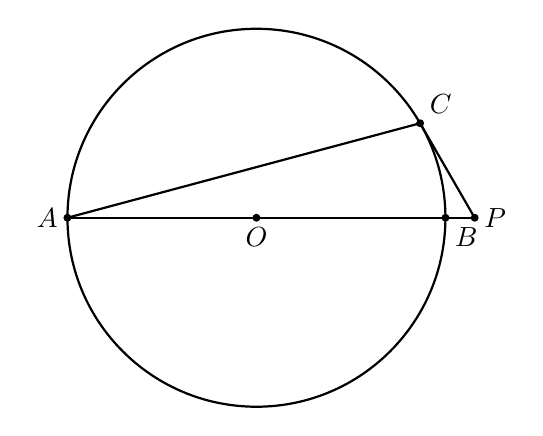
\begin{tikzpicture}[scale=1.2]
  \coordinate (O) at (0,0);
  \coordinate (A) at (-2,0);
  \coordinate (B) at (2,0);
  \coordinate (C) at (1.732,1);
  \coordinate (P) at (2.309,0);
  \draw[thick] (O) circle (2);
  \draw[thick] (A)--(P);
  \draw[thick] (A)--(C);
  \draw[thick] (C)--(P);
  \fill (O) circle (1.2pt) node[below] {$O$};
  \fill (A) circle (1.2pt) node[left] {$A$};
  \fill (B) circle (1.2pt) node[below right] {$B$};
  \fill (C) circle (1.2pt) node[above right] {$C$};
  \fill (P) circle (1.2pt) node[right] {$P$};
\end{tikzpicture}
\end{center}
\nopagebreak[4]
\gkanswer{答案：半径为 $12\sqrt{3}\ \mathrm{cm}$。}

\end{answer}
\begin{answer}
\gksolhead{7}{}

\textbf{题目}：

设直线 $l_{1}$ 和 $l_{2}$ 的斜率是方程 $6x^{2}-x-1=0$ 的两个根，求直线 $l_{1}$ 和 $l_{2}$ 的交角。

\Needspace{4\baselineskip}
\textbf{解析}

\Needspace{5\baselineskip}
方程 $6x^{2}-x-1=0$ 的两根为

\nopagebreak[4]
\[
x=\frac{1\pm\sqrt{1+24}}{12}=\frac{1\pm5}{12},
\qquad
k_{1}=\frac{1}{2},\quad k_{2}=-\frac{1}{3}.
\]

\Needspace{5\baselineskip}
设两直线交角为 $\varphi$，则

\nopagebreak[4]
\[
\tan\varphi
=\left|\frac{k_{1}-k_{2}}{1+k_{1}k_{2}}\right|
=\frac{\dfrac{1}{2}+\dfrac{1}{3}}{1-\dfrac{1}{6}}
=\frac{\dfrac{5}{6}}{\dfrac{5}{6}}=1,
\qquad
\varphi=45^{\circ}.
\]

\gkanswer{答案：$45^{\circ}$。}

\end{answer}
\begin{answer}
\gksolhead{8}{}

\textbf{题目}：

把极坐标方程 $\rho=4\sin\theta$ 化为直角坐标方程。

\Needspace{4\baselineskip}
\textbf{解析}

\Needspace{5\baselineskip}
$\rho=4\sin\theta$ 两边同乘 $\rho$，得 $\rho^{2}=4\rho\sin\theta$。由 $x^{2}+y^{2}=\rho^{2}$，$y=\rho\sin\theta$，故

\nopagebreak[4]
\[
x^{2}+y^{2}=4y,
\qquad\text{\text{即}}\qquad
x^{2}+(y-2)^{2}=4.
\]

（极点 $\rho=0$ 满足原方程，且已含于该圆。）

\gkanswer{答案：$x^{2}+y^{2}-4y=0$，即 $x^{2}+(y-2)^{2}=4$。}

\end{answer}
\begin{answer}
\gksolhead{9}{}

\textbf{题目}：

甲乙两地相距 12 公里，一货船由甲地顺流航行到乙地装货，返航时每小时速度减少了 4 公里，因此比去时多用了 30 分钟，求该船去时速度。

\Needspace{4\baselineskip}
\textbf{解析}

\Needspace{5\baselineskip}
设该船去时速度为 $v$ 公里/小时（$v>4$），则返航速度为 $v-4$ 公里/小时。多用的 30 分钟即 $\dfrac{1}{2}$ 小时：

\nopagebreak[4]
\[
\frac{12}{v-4}-\frac{12}{v}=\frac{1}{2}
\quad\Longrightarrow\quad
\frac{48}{v(v-4)}=\frac{1}{2}
\quad\Longrightarrow\quad
v^{2}-4v-96=0.
\]

解得 $v=12$ 或 $v=-8$（舍去）。故该船去时速度为 $12$ 公里/小时。

\gkanswer{答案：该船去时速度为 $12$ 公里/小时。}

\end{answer}
\begin{answer}
\gksolhead{10}{}

\textbf{题目}：

在 $\triangle ABC$ 中，$\angle A$ 的正切是 2，$\angle B$ 的正切是 3，

（1） 求 $\angle C$ 的正切；

（2） 这个三角形是钝角三角形、锐角三角形、还是直角三角形？为什么？

（3） 设这个三角形最短边是 1，求它的最长边。

\Needspace{4\baselineskip}
\textbf{解析}

\gksubpart{（1）}

\nopagebreak[4]
\[
\tan C=-\tan(A+B)
=-\frac{\tan A+\tan B}{1-\tan A\tan B}
=-\frac{2+3}{1-2\times3}=1.
\]

\gksubpart{（2）}

\Needspace{5\baselineskip}
$\tan A=2>0$，$\tan B=3>0$，故 $A$、$B$ 均为锐角；由 $\tan(A+B)=-1$ 且 $0^{\circ}<A+B<180^{\circ}$，得 $A+B=135^{\circ}$，从而

\nopagebreak[4]
\[
C=180^{\circ}-135^{\circ}=45^{\circ},
\]

也是锐角。所以 $\triangle ABC$ 是锐角三角形。

\gksubpart{（3）}

\Needspace{5\baselineskip}
$\tan A=2$，$\tan B=3$，$\tan C=1$，各角为 $A\approx63.43^{\circ}$，$B\approx71.57^{\circ}$，$C=45^{\circ}$。最小角 $C$ 所对的边 $c$ 最短（即 $c=1$），最大角 $B$ 所对的边 $b$ 最长。由 $\tan B=3$ 得 $\sin B=\dfrac{3}{\sqrt{10}}$，又 $\sin C=\dfrac{\sqrt{2}}{2}$，由正弦定理

\nopagebreak[4]
\[
b=\frac{c\sin B}{\sin C}
=\frac{1\times\dfrac{3}{\sqrt{10}}}{\dfrac{\sqrt{2}}{2}}
=\frac{3}{\sqrt{5}}
=\frac{3\sqrt{5}}{5}.
\]

所以最长边为 $\dfrac{3\sqrt{5}}{5}$。

\gkanswer{答案（1）：$\tan C=1$。}

\gkanswer{答案（2）：锐角三角形（$\angle C=45^{\circ}$，三个内角均为锐角）。}

\gkanswer{答案（3）：最长边为 $\dfrac{3\sqrt{5}}{5}$。}

\end{answer}